%\documentclass[french]{beamer}
\documentclass[aspectratio=169]{beamer}
\usepackage[utf8]{inputenc}
\usepackage[T1]{fontenc}
\usepackage{lmodern}
\usepackage{amsmath, amssymb}
\usepackage{babel}

\usepackage{eurosym}
%\usepackage{unicode-math}
\setbeamertemplate{footline}[frame number]
\def\checkmark{\tikz\fill[scale=0.4](0,.35) -- (.25,0) -- (1,.7) -- (.25,.15) -- cycle;} 
\definecolor{rouge}{HTML}{DD0000}

%Pour le TITLEPAGE

\title{Appel à projet - Présentation}
\subtitle{\today}
\date{}
\author[N.P. - A.M. - P.T.]{Nicolas Papazoglou, Alexis Martin \& Pierre Toussaint}
\institute[ENSEA]{ENSEA}

\usetheme{ensea}  

\begin{document}

\begin{frame}
	\titlepage
\end{frame}

\begin{frame}{Rappel}
\begin{minipage}{0.49\textwidth}
	\begin{itemize}
		\item Porteurs du projet : Nicolas Papazoglou, Alexis Martin, Pierre Toussaint,
		\item Demande budgétaire : 64 HETD, 
		\item Budget (DEE) : 400-500\euro/maquette,
		\item Activités concernées : enseignements d'électrotechnique et d'automatique.
	\end{itemize}
\end{minipage}
\begin{minipage}{0.49\textwidth}
	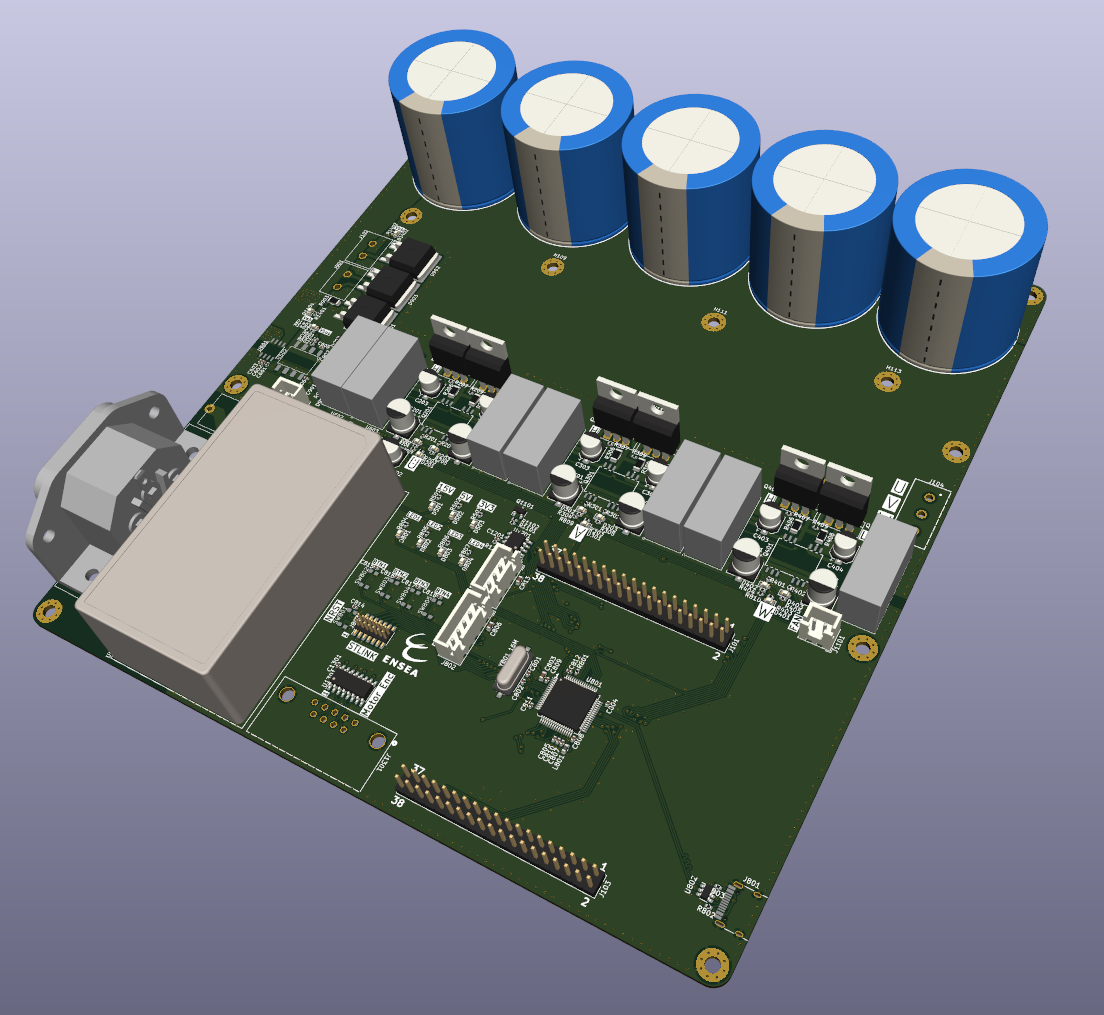
\includegraphics[width=0.9\textwidth]{figures/inverter.png} 
\end{minipage}
\center \href{https://github.com/DBXYD/AAP_ENSEA_Inverter}{Lien github}
\end{frame}

%********************** OBJECTIFS ******************************
\begin{frame}{Contexte}
\begin{itemize}
	\item Maquette de TP : onduleur triphasé,
	\item TP en 3eme année (Enseignements d'électrotechnique et d'automatique) : 
	\begin{itemize}
	\item [ESE\_3745] Actionneur et automatique appliquée
	\item [MSC\_3805] Systèmes d'Acquision et de commande
	\end{itemize}
	\item 12 maquettes obsolète Powermodule MC1L 3-Phase (Microchip) : 
	\item Pannes récurentes :
	\begin{itemize}
		\item Perte de temps pour les étudiants,
		\item Recherche de panne et réparation par les professeurs,
		\item Boite noire pour les étudiants.		
	\end{itemize}
\end{itemize}
\end{frame}

\begin{frame}{Objectif : Réalisation maquette pédagogique}
	Objectifs : 
	\begin{enumerate}
		\item Une maquette fiable pour les TPs d'électrotechnique et automatique \\
		$\rightarrow$ Gain en temps et en autonomie pour les étudiants, \checkmark
		\item Feedback automatique en fonction des erreurs détectées, \\
		$\rightarrow$ Gain en autonomie pour les étudiants, possibilité de travail hors séance sans supervision d'un professeur,
		\item Projet open-source (disponible sur \href{https://github.com/DBXYD/AAP_ENSEA_Inverter}{github}), \checkmark
		\item Compréhension globale possible par les étudiants, application de l'ensemble de leurs cours dans une maquette, \checkmark
		\item Création modulaire, réutilisable dans d'autres cours/projets,  \checkmark
		\item Evolution possible à d'autres enseignements (buck/boost, 4Q, brushless, moteurs synchrones, asservissement, etc...), \checkmark
		\item Maintenance facile et rapide. \checkmark
	\end{enumerate}
\end{frame}



\begin{frame}{Bilan}
\begin{enumerate}
	\item Cahier des charges \checkmark,
	\item Schéma d'architecture \checkmark,
	\item Choix des composants \checkmark,
	\item Prototypage et tests unitaires électriques \checkmark,
	\item Réalisation software et tests complets (50\%),
	\item Réalisation mécanique (boitier) (50\%),
	\item Documentation (\href{https://github.com/DBXYD/AAP_ENSEA_Inverter}{github}). (80\%)
\end{enumerate}
\pause
Remarque :\begin{itemize}
	\item Coût : 300\euro/maquette,
	\item 8 cartes en fabrication dans l'immédiat
	\item Beaucoup de composants gratuits
\end{itemize}	
\end{frame}

\begin{frame}{Schematic}
\begin{center}
	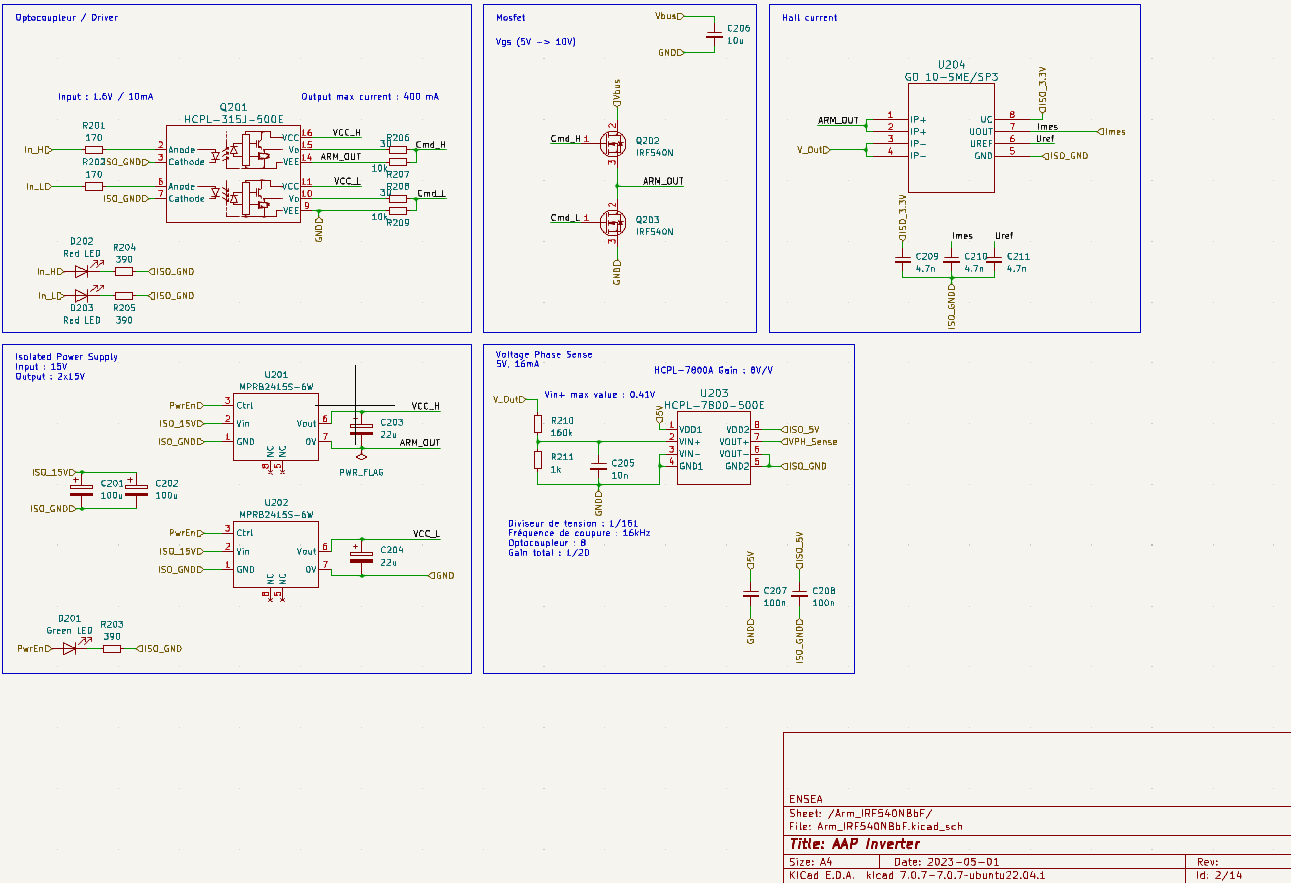
\includegraphics[width=0.7\textwidth]{figures/schematic.png} 
\end{center}
\end{frame}

\begin{frame}{PCB}
\begin{minipage}{0.49\textwidth}
\begin{center}
	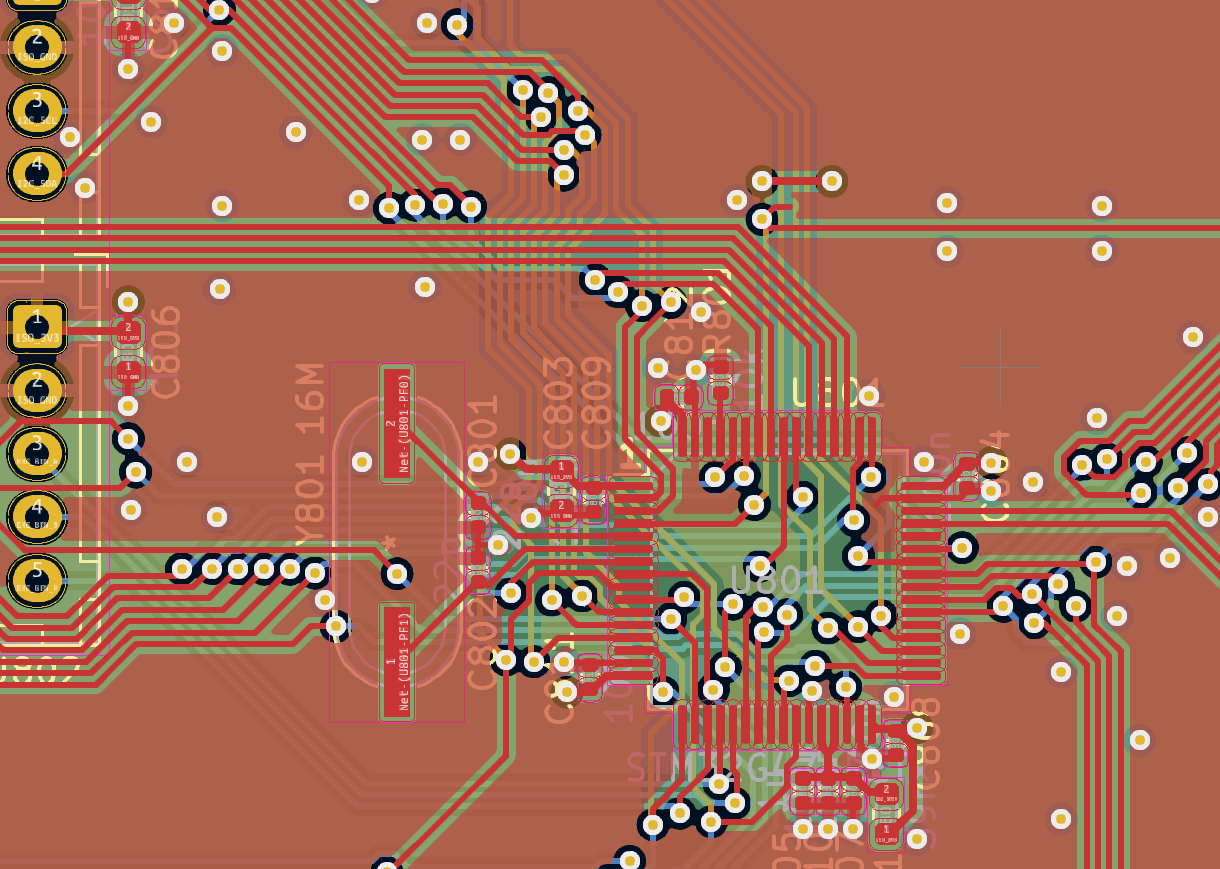
\includegraphics[width=0.9\textwidth]{figures/pcb.png} 
\end{center}
\end{minipage}
\begin{minipage}{0.49\textwidth}
\begin{itemize}
	\item 242 composants (60 différents),
	\item 2000 segments de pistes,
	\item 906 pads
	\item 225 signaux
\end{itemize}
\end{minipage}
\end{frame}

\begin{frame}{La suite}
\begin{minipage}{0.39\textwidth}
\begin{center}
	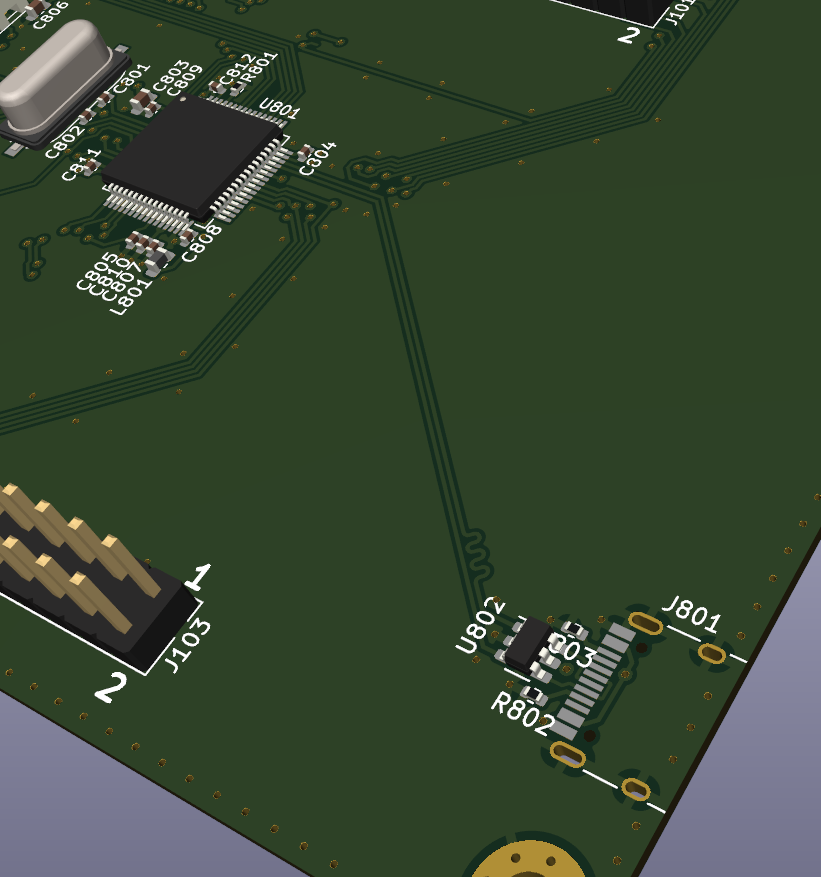
\includegraphics[width=0.9\textwidth]{figures/usb.png} 
\end{center}
\end{minipage}
\begin{minipage}{0.59\textwidth}
Idée 1 : 
\begin{itemize}
	\item Connexion usb fonctionnelle
	\item Possibilité de récupérer toutes les données internes
	\item Programme et interface (Python) pour afficher de façon didactique l'état du moteur
\end{itemize}
Idée 2 : 
\begin{itemize}
	\item Possibilité de TP de puissance à distance
\end{itemize}
Idée 3 : 
\begin{itemize}
	\item Portage de ce projet sur d'autres cours 
	\item Carte fille différente (remplacement de la Nucléo)
\end{itemize}
\end{minipage}
\end{frame}


\end{document}